\documentclass[12pt]{article}
\usepackage[spanish]{babel}
\usepackage[utf8]{inputenc}
\usepackage{geometry}
\usepackage{graphicx}
\usepackage{hyperref}
\usepackage{setspace}
\usepackage{tocloft}
\usepackage{booktabs}
\usepackage{listings}

\geometry{margin=2.5cm}
\setstretch{1.5}
\lstset{basicstyle=\ttfamily\small, breaklines=true}

% ------------------------------------------------
% PORTADA
% ------------------------------------------------
\begin{document}
\begin{titlepage}
    \centering

    {\scshape\LARGE Universidad del Valle de Guatemala \par}
    \vspace{1cm}
    {\scshape\Large Facultad de Ingeniería \par}
    {\scshape\Large Departamento de Ciencias de la Computación \par}
    \vspace{1.5cm}
    {\huge\bfseries Proyecto 2: Análisis Exploratorio de Datos \par}
    \vspace{0.5cm}
    {\Large Tema 12: Reconocimiento de deletreo manual en Lengua de Señas Americana (ASL) \par}
    \vspace{2cm}
    {\Large Curso: CC3084 – Data Science \par}
    \vfill
    {\Large Integrantes del grupo: \par}
    \begin{tabular}{l}
        - Diederich Solis 22952 \\
        - Juan Cordón \\
        - Sebas Juarez \\
        - Sara Guzman \\
    \end{tabular}
    \vfill
    {\Large Semestre II – 2025 \par}
\end{titlepage}

% ------------------------------------------------
% ÍNDICE
% ------------------------------------------------
\tableofcontents
\newpage

% ------------------------------------------------
% INTRODUCCIÓN
% ------------------------------------------------
\section{Introducción}
La lengua de señas constituye el medio principal de comunicación para más de 70 millones de personas sordas en el mundo, y se estima que más de 1500 millones de personas padecen algún grado de pérdida auditiva \cite{who_hearing}.  
El \textit{American Sign Language} (ASL) es el sistema más comúnmente utilizado en los Estados Unidos, y dentro de este, el \textbf{deletreo manual} cumple un papel fundamental para expresar nombres propios, direcciones, números y otros términos que no cuentan con un signo específico.

El reto tecnológico consiste en que, a diferencia del reconocimiento automático de voz o la traducción de texto, los sistemas de inteligencia artificial para el reconocimiento del ASL aún se encuentran en desarrollo. La principal dificultad radica en la complejidad de los gestos, las variaciones individuales entre usuarios y la falta de conjuntos de datos suficientemente grandes y diversos.  

Este informe busca analizar de manera exploratoria un conjunto de datos de deletreo manual en ASL, con el fin de establecer las bases para futuros modelos de reconocimiento automático basados en visión por computadora.

% ------------------------------------------------
% PLANTEAMIENTO INICIAL DEL PROBLEMA
% ------------------------------------------------
\section{Planteamiento inicial del problema}

\subsection{Situación problemática}
Los avances en inteligencia artificial han revolucionado el reconocimiento automático de voz y la traducción de texto, facilitando la interacción entre humanos y dispositivos. Sin embargo, estos desarrollos aún no se he extendido plenamente al ámbito de la lengua de señas, lo que genera una brecha tecnológica para millones de personas sordas.  

El deletreo manual del ASL permite formar palabras letra por letra mediante configuraciones específicas de la mano. En la vida cotidiana, se utiliza para introducir información esencial como nombres propios, direcciones de correo electrónico, números de teléfono o acrónimos. Muchos usuarios sordos de teléfonos inteligentes pueden deletrear palabras con sus manos de manera más rápida que escribir en teclados virtuales, alcanzando hasta 57 palabras por minuto frente a un promedio de 36 en usuarios oyentes \cite{asl_speed}.  

No obstante, los sistemas automáticos de reconocimiento del deletreo manual aún presentan desafíos:  
\begin{itemize}
    \item Variabilidad entre usuarios (tamaño de manos, estilo personal, destreza).  
    \item Diferencias en condiciones de captura (iluminación, ángulos de cámara, accesorios).  
    \item Falta de representatividad en los datos (pocos tonos de piel, predominio de usuarios de ciertas regiones).  
\end{itemize}

\subsection{Problema científico}
Derivado de lo anterior surge la siguiente pregunta de investigación:  
\begin{quote}
    \textbf{¿Es posible desarrollar un modelo de visión por computadora que reconozca con precisión el deletreo manual del lenguaje de señas estadounidense (ASL), a partir de imágenes y metadatos recolectados en condiciones reales de uso, considerando la variabilidad entre usuarios y los posibles sesgos del dataset?}
\end{quote}

\subsection{Objetivos}

\subsubsection*{Objetivo general}
Analizar de manera exploratoria el conjunto de datos de deletreo manual en ASL con el fin de sentar las bases para un modelo de reconocimiento automático que contribuya a la accesibilidad tecnológica para personas sordas y con pérdida auditiva.

\subsubsection*{Objetivos específicos}
\begin{enumerate}
    \item Describir y caracterizar el dataset de ASL Fingerspelling, identificando variables, estructura y calidad de los datos.
    \item Implementar procesos de limpieza y preprocesamiento que aseguren la consistencia de la información.
    \item Realizar un análisis estadístico y visual de los datos para detectar patrones, desbalances y posibles sesgos.
    \item Establecer implicaciones y lineamientos para la construcción de modelos de clasificación basados en visión artificial.
\end{enumerate}

% ------------------------------------------------
% DESCRIPCIÓN DE LOS DATOS
% ------------------------------------------------
\section{Descripción de los datos}

\subsection{Origen de los datos}
El conjunto de datos utilizado en este proyecto fue recolectado con la participación de más de \textbf{100 personas usuarias de la Lengua de Señas Americana (ASL)} en distintas regiones de Estados Unidos. Todas las personas participantes fueron reclutadas a través de la Red de Artes Profesionales para Sordos, garantizando que el ASL fuera su lengua materna y principal medio de comunicación. Esta diversidad aporta variabilidad en características físicas, tonos de piel y estilos de deletreo, lo que enriquece la representatividad del dataset.

\subsection{Proceso de recopilación}
La recopilación de datos se realizó mediante \textbf{smartphones} que incluían una aplicación especialmente diseñada para registrar secuencias de video. Cada participante debía presionar un botón para iniciar y finalizar la grabación, durante la cual \textbf{deletreaban en ASL} el texto que aparecía en la pantalla.  
Las condiciones de captura fueron intencionalmente diversas para reflejar escenarios reales de uso:
\begin{itemize}
    \item \textbf{Variación en las manos:} algunos participantes utilizaron la mano izquierda, otros la derecha, e incluso alternaron entre ambas en diferentes secuencias.
    \item \textbf{Variación postural y de encuadre:} diferencias en distancia a cámara, zoom, pose corporal, iluminación y presencia de accesorios.
    \item \textbf{Frases objetivo:} palabras, nombres y direcciones que normalmente se introducen en dispositivos móviles, reflejando un uso práctico del deletreo manual.
\end{itemize}

\subsection{Contenido del dataset}
Para efectos de este proyecto únicamente se utilizará el archivo \textbf{\texttt{supplemental\_metadata.csv}}, ya que contiene la información necesaria para realizar el análisis exploratorio solicitado. Este archivo incluye variables descriptivas de las secuencias capturadas, sin necesidad de procesar los archivos de landmarks (\texttt{.parquet}) debido a su gran tamaño y complejidad, lo cual excede el alcance de esta entrega.  

Las variables principales contenidas en el archivo de metadatos son:
\begin{itemize}
    \item \texttt{path}: ruta o identificador del archivo de referencia.
    \item \texttt{file\_id}: identificador único del archivo.
    \item \texttt{participant\_id}: identificador de la persona firmante.
    \item \texttt{sequence\_id}: identificador de la secuencia de video.
    \item \texttt{phrase}: palabra o frase deletreada en la secuencia.
\end{itemize}

\subsection{Variables categóricas}
Existen varias variables categóricas de interés para el análisis:
\begin{itemize}
    \item \texttt{participant\_id}: identifica a la persona que firma. Permite estudiar variaciones entre usuarios.
    \item \texttt{phrase}: corresponde a la palabra deletreada. Puede descomponerse en letras individuales para análisis de balance de clases.
    \item \texttt{letter}: variable derivada que representa cada carácter del alfabeto manual.
\end{itemize}

\subsection{Estructura general}
En la Tabla~\ref{tab:variables} se resumen las principales variables del archivo \texttt{supplemental\_metadata.csv}.

\begin{table}[h]
\centering
\caption{Resumen de variables principales del archivo de metadatos}
\label{tab:variables}
\begin{tabular}{@{}lll@{}}
\toprule
\textbf{Variable} & \textbf{Tipo} & \textbf{Descripción} \\ \midrule
\texttt{participant\_id} & Categórica & ID anónimo del participante. \\
\texttt{sequence\_id} & Entera & ID único de secuencia. \\
\texttt{file\_id} & Entera & Identificador único del archivo. \\
\texttt{path} & Texto & Ruta del archivo de referencia. \\
\texttt{phrase} & Categórica & Palabra o frase deletreada. \\
\bottomrule
\end{tabular}
\end{table}



\subsection{Estructura y dimensiones}
El archivo \texttt{supplemental\_metadata.csv} contiene un total de \textbf{43,998 secuencias} y \textbf{509 frases distintas}, asociadas a los participantes mediante identificadores únicos. No se detectaron valores nulos en las variables principales (\texttt{path}, \texttt{file\_id}, \texttt{sequence\_id}, \texttt{participant\_id}, \texttt{phrase}), lo que indica una buena calidad de datos a nivel de metadatos.

\subsection{Distribución de frases}
El análisis inicial muestra que las frases más frecuentes en el dataset incluyen expresiones como \textit{“find a nearby parking spot”} y \textit{“most judges are very honest”}, cada una con más de 100 repeticiones. Estas frases reflejan ejemplos de lenguaje cotidiano que suelen escribirse en dispositivos móviles, lo que confirma la intención práctica del conjunto de datos.

\subsection{Distribución por letras}
A partir de las frases se derivó la variable \texttt{letter}, correspondiente a la primera letra de cada palabra o frase deletreada. 

\begin{figure}[h]
    \centering
    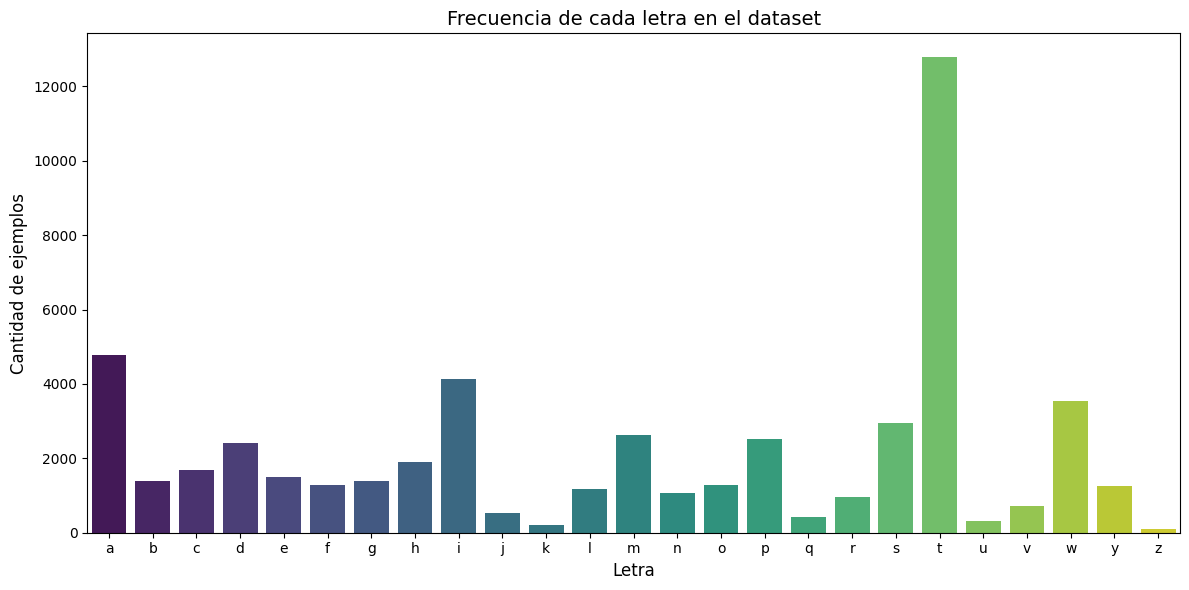
\includegraphics[width=0.95\textwidth]{grafico_letras.png}
    \caption{Distribución de secuencias por letra derivada de las frases.}
    \label{fig:letras}
\end{figure}

La Figura~\ref{fig:letras} muestra la distribución de secuencias por letra. Se observa un fuerte desbalance de clases:  
\begin{itemize}
    \item La letra \textbf{t} concentra más de 10,000 ejemplos, representando casi una cuarta parte del total.
    \item Letras como \textbf{z} (87 ejemplos), \textbf{k} (180 ejemplos) y \textbf{q} (338 ejemplos) aparecen con muy baja frecuencia.
    \item Otras letras como \textbf{a} (3,980), \textbf{i} (3,398) y \textbf{w} (2,959) están mejor representadas.
\end{itemize}

Este desbalance tendrá implicaciones importantes en fases posteriores de modelado, donde será necesario aplicar técnicas de balanceo o ponderación de clases.

\subsection{Distribución por participantes}

\begin{figure}[h]
    \centering
    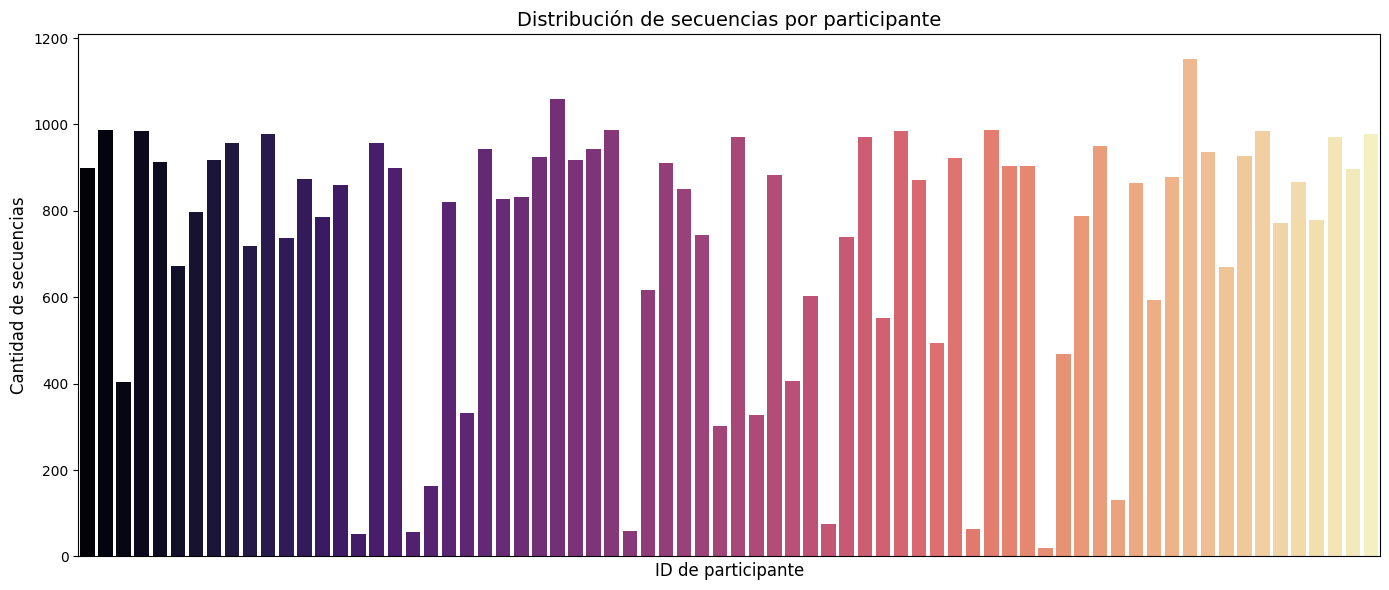
\includegraphics[width=0.95\textwidth]{grafico_participantes.png}
    \caption{Distribución de secuencias por participante.}
    \label{fig:participantes}
\end{figure}

La Figura~\ref{fig:participantes} muestra la distribución de secuencias por participante. Se observa que:  
\begin{itemize}
    \item La participación no es homogénea: algunos usuarios aportaron más de 900 secuencias, mientras que otros contribuyeron con menos de 200.
    \item Esto introduce un \textbf{sesgo potencial}, ya que un pequeño grupo de participantes podría dominar el entrenamiento de futuros modelos.
    \item Aun así, la variedad de 72 personas firmantes constituye un avance frente a datasets más pequeños o menos diversos.
\end{itemize}

\subsection{Notas preliminares}
Los hallazgos de esta sección resaltan dos características clave del dataset:  
\begin{enumerate}
    \item Existe un \textbf{desbalance significativo entre letras}, lo cual podría sesgar modelos de clasificación hacia las clases mayoritarias.  
    \item La \textbf{contribución desigual de los participantes} puede limitar la generalización si no se controla durante el entrenamiento.  
\end{enumerate}
Estos aspectos serán abordados en la fase de limpieza y preprocesamiento, donde se definirán estrategias de normalización y balanceo de datos.

\section{Limpieza y Preprocesamiento de los datos}

\subsection{Estrategia general}
El conjunto de datos analizado presenta buena calidad en cuanto a completitud, ya que no se detectaron valores nulos en las variables principales. Sin embargo, el análisis exploratorio reveló dos aspectos críticos que deben atenderse antes de su uso en fases posteriores de modelado:

\begin{enumerate}
    \item \textbf{Desbalance de clases:} se observó que algunas letras (\textit{t}, \textit{a}, \textit{i}, \textit{w}) concentran un número muy elevado de ejemplos, mientras que otras (\textit{z}, \textit{k}, \textit{q}) tienen muy pocas instancias. Esto puede sesgar los modelos hacia clases mayoritarias.
    \item \textbf{Contribución desigual de participantes:} algunos usuarios aportaron más de 900 secuencias, mientras que otros menos de 200. Esto podría introducir un sesgo hacia ciertos estilos de señado.
\end{enumerate}

\subsection{Acciones de limpieza propuestas}
Para garantizar consistencia y robustez en la información, se definieron las siguientes acciones de limpieza y preprocesamiento:

\begin{itemize}
    \item \textbf{Normalización de texto:} transformar todas las frases a minúsculas y eliminar espacios en blanco al inicio y final para evitar duplicidades.
    \item \textbf{Derivación de variable categórica \texttt{letter}:} generar la columna correspondiente a la primera letra de cada frase, con el fin de estudiar la distribución de clases y su equilibrio.
    \item \textbf{Validación de claves:} comprobar que no existan duplicados en los identificadores \texttt{sequence\_id} y \texttt{file\_id}, asegurando unicidad de cada observación.
    \item \textbf{Chequeo de valores faltantes:} aunque no se detectaron inicialmente, se verificará sistemáticamente la presencia de celdas vacías o inconsistencias en las columnas principales.
    \item \textbf{Análisis de balance de clases:} calcular la frecuencia relativa de cada letra para identificar el nivel de desbalance y documentar sus implicaciones.
    \item \textbf{Análisis de distribución por participante:} revisar si existen participantes con muy baja contribución (outliers) que podrían distorsionar el entrenamiento de modelos.
\end{itemize}



\subsection{Resultados de la limpieza y preprocesamiento}



\begin{figure}[h]
    \centering
    \includegraphics[width=0.95\textwidth]{resultadoslimpieza.png}
    \caption{Resultado limpieza.}
    \label{fig:limpieza}
\end{figure}


La Figura~\ref{fig:limpieza} Tras aplicar las acciones de limpieza propuestas, se obtuvieron los siguientes hallazgos clave: 



\begin{itemize}
    \item \textbf{Duplicados:} No se encontraron duplicados en los identificadores \texttt{sequence\_id}, lo que confirma que cada secuencia es única. En el caso de \texttt{file\_id}, se observaron coincidencias debido a que varios fragmentos pueden provenir del mismo archivo de video, lo cual es consistente con el diseño del dataset.
    \item \textbf{Valores nulos:} Ninguna de las variables analizadas (\texttt{path}, \texttt{file\_id}, \texttt{sequence\_id}, \texttt{participant\_id}, \texttt{phrase}, \texttt{letter}) presentó valores faltantes, lo que refuerza la completitud y calidad de los metadatos.
    \item \textbf{Dimensiones finales:} El conjunto limpio cuenta con \textbf{52,958 secuencias}, \textbf{509 frases distintas} y \textbf{72 participantes}.
\end{itemize}

\subsubsection*{Distribución por letras}
El análisis de la variable \texttt{letter} revela un desbalance significativo:
\begin{itemize}
    \item La letra \textbf{t} concentra el 24.1\% de todas las secuencias (12,790 instancias).
    \item Otras letras como \textbf{a} (9.0\%), \textbf{i} (7.8\%) y \textbf{w} (6.6\%) también aparecen con alta frecuencia.
    \item En contraste, letras como \textbf{z} (104 ejemplos), \textbf{k} (216) y \textbf{u} (321) están muy poco representadas, con proporciones inferiores al 1\%.
\end{itemize}

El \textbf{índice de Gini calculado para la distribución de letras fue 0.487}, lo que refleja un nivel de desbalance medio-alto (donde 0 indica perfecta equidad y 1 desbalance extremo). Esto implica que los modelos entrenados con este dataset tenderían a sesgarse hacia letras mayoritarias si no se aplican técnicas de balanceo.

\subsubsection*{Distribución por participantes}
La contribución de los 72 participantes también muestra cierta desigualdad:
\begin{itemize}
    \item En promedio, cada persona aportó unas \textbf{735 secuencias}, con una desviación estándar de 295.
    \item El rango va desde un mínimo de solo \textbf{20 secuencias} hasta un máximo de \textbf{1,151 secuencias}.
    \item Este comportamiento sugiere que algunos estilos de señado están más representados que otros, lo cual puede introducir un sesgo hacia participantes con mayor volumen de datos.
\end{itemize}

\subsection{Implicaciones para el modelado}
El análisis de limpieza y preprocesamiento permite concluir que, aunque el dataset presenta buena calidad estructural y no requiere correcciones mayores, los \textbf{problemas de desbalance entre letras y participantes} deben abordarse en etapas posteriores.

% ------------------------------------------------
% ANÁLISIS ESTADÍSTICO / EXPLORATORIO
% ------------------------------------------------

\section{Análisis estadístico}

Para entender mejor los datos, hicimos un análisis más profundo viendo:
\begin{itemize}
    \item Estadísticas descriptivas de las variables numéricas y categóricas.
    \item Revisión de valores faltantes.
    \item Análisis de correlaciones entre variables numéricas.
    \item Búsqueda de posibles outliers.
\end{itemize}

No encontramos valores faltantes importantes y las variables numéricas principales no muestran correlaciones fuertes entre sí, lo cual es normal porque son identificadores. Los boxplots muestran que los datos están bastante bien distribuidos y no hay outliers extremos.

También agregamos dos gráficas clave para el contexto de ASL:
\begin{itemize}
    \item Frecuencia de cada letra en el dataset.
    \item Distribución de secuencias por participante.
\end{itemize}

\begin{figure}[h]
    \centering
    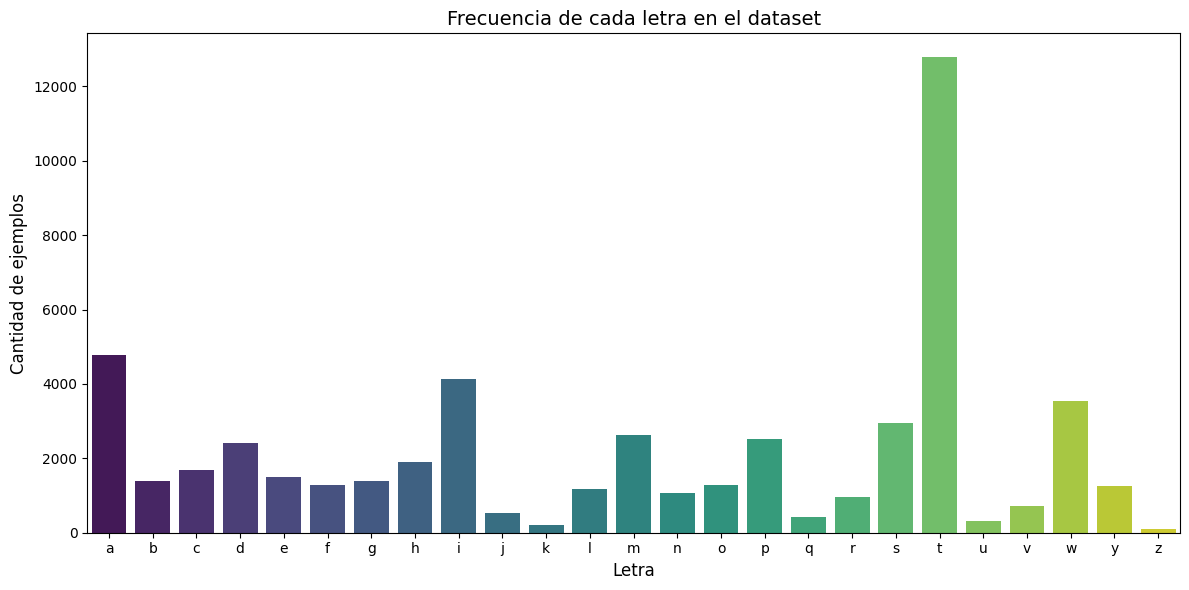
\includegraphics[width=0.95\textwidth]{grafico_letras.png}
    \caption{Frecuencia de cada letra en el dataset.}
    \label{fig:letras2}
\end{figure}

\begin{figure}[h]
    \centering
    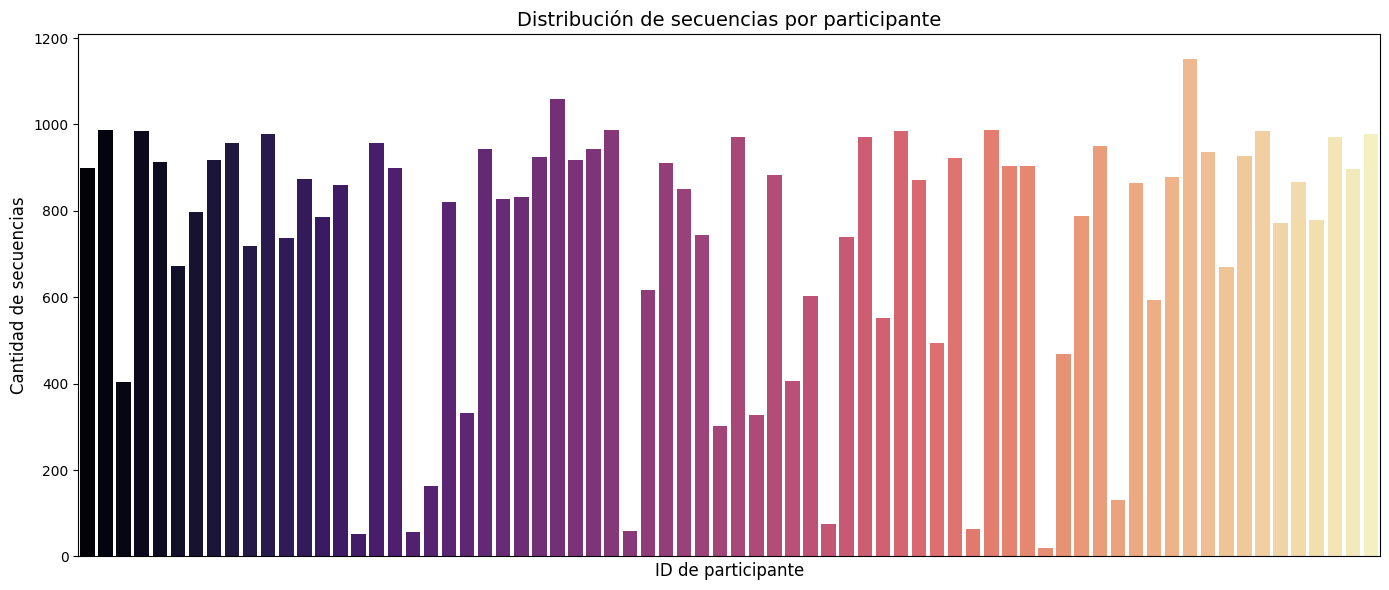
\includegraphics[width=0.95\textwidth]{grafico_participantes.png}
    \caption{Distribución de secuencias por participante.}
    \label{fig:participantes2}
\end{figure}

\subsection*{Conclusiones}
\begin{enumerate}
    \item Hay letras que aparecen mucho más que otras en el dataset. Si entrenamos un modelo así, va a aprender mejor las letras más comunes y puede fallar con las menos usadas. Por eso, es importante balancear los datos antes de entrenar.
    \item Algunos participantes aportaron muchas más secuencias que otros. Si no cuidamos esto, el modelo podría aprender a reconocer mejor a ciertos usuarios y no funcionar tan bien con personas nuevas. Es mejor asegurarse de que el modelo sea justo para todos.
\end{enumerate}

% ------------------------------------------------
% VISUALIZACIÓN DE SEÑAS Y DISTRIBUCIONES
% ------------------------------------------------

\section{Visualización de señas y distribuciones}

A continuación se muestran ejemplos visuales de cómo se representan algunas letras del alfabeto en ASL, usando imágenes de manos reales del dataset:

\begin{figure}[h]
    \centering
    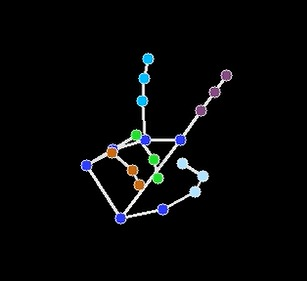
\includegraphics[width=0.22\textwidth]{Mano1.png}
    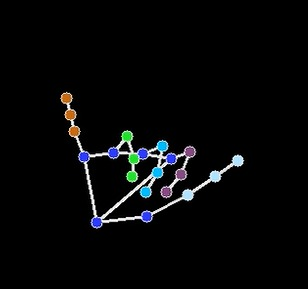
\includegraphics[width=0.22\textwidth]{Mano2.png}
    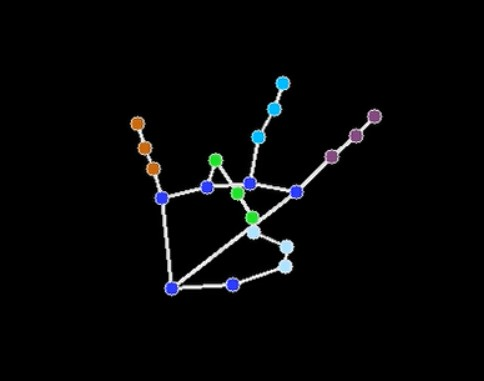
\includegraphics[width=0.22\textwidth]{Mano3.png}
    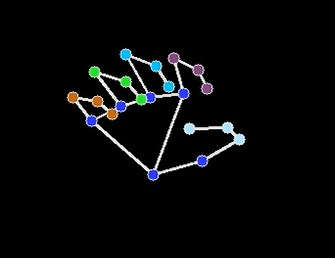
\includegraphics[width=0.22\textwidth]{Mano4.png}
    \caption{Ejemplos de señas manuales para letras en ASL extraídas del dataset.}
    \label{fig:manos_asl}
\end{figure}

También se incluyen los boxplots de las variables numéricas principales, que ayudan a visualizar la distribución y posibles valores atípicos en los datos:

\begin{figure}[h]
    \centering
    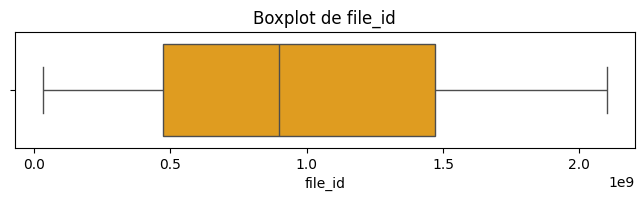
\includegraphics[width=0.32\textwidth]{Box_fiel.png}
    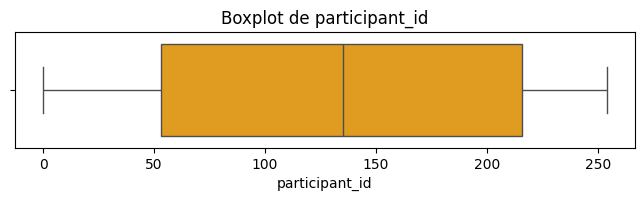
\includegraphics[width=0.32\textwidth]{Box_participant.png}
    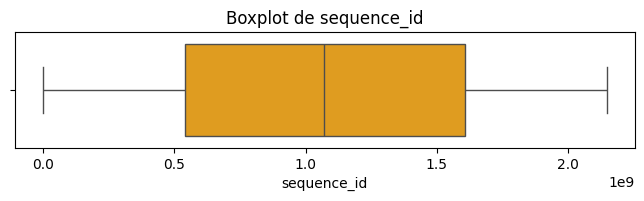
\includegraphics[width=0.32\textwidth]{Box_sequence.png}
    \caption{Boxplots de las variables file	extunderscore id, participant	extunderscore id y sequence	extunderscore id. No se observan outliers extremos.}
    \label{fig:boxplots}
\end{figure}

% ------------------------------------------------
% BIBLIOGRAFÍA
% ------------------------------------------------
\newpage
\begin{thebibliography}{9}
\bibitem{who_hearing} World Health Organization (2021). \textit{World Report on Hearing}. Disponible en: \url{https://www.who.int/publications/i/item/world-report-on-hearing}
\bibitem{asl_speed} Goldin-Meadow, S. (2010). \textit{The Resilience of Language: What Gesture Creation in Deaf Children Can Tell Us About How All Children Learn Language}. Psychology Press.
\end{thebibliography}

\end{document}